% !TeX spellcheck = it_IT

\section{Strutture succinte, quasi-succinte e compatte}
Abbiamo lavorato con dei razzi, ora si parla di oggetti estremamente piccoli, strutture dati molto semplici.\\

Intanto, cos'è una struttura dati? Intendiamo un \textbf{Abstract Data Type ADT}, ovvero un \textbf{insieme di primitive}, ad esempio su uno stack le primitive potrebbero essere \texttt{push}, \texttt{pop} e \texttt{is\_empty}. Esistono modi formali, assiomatici, per definire le ADT.\\

Ogni ADT si può implementare e possono esserci molte \textbf{implementazioni} diverse, che funzionalmente corrispondono alla stessa ADT, ma differiscono per \textbf{complessità in spazio e tempo}.\\

\subsection{Information-Theoretical Lower Bound}

Supponendo di avere una struttura dati specifica che per \textbf{taglia} $n$ abbia $V_n$ \textbf{valori possibili}, che chiameremo: 
$$ v_1, v_2, \, \dots \, , v_{V_n} $$

Ed ognuno di questi possibili \textbf{valori} utilizza un \textbf{certo numero di bit}
$$ x_1, x_2, \, \dots \, , x_{V_n}$$

Allora il \textbf{teorema di Shannon} dice che
$$ \frac{x_1 + x_2 + \, \dots \, + x_{V_n}}{V_n} \geq \log_2 V_n $$

Sostanzialmente, la \textbf{media delle dimensione di tutti i valori} non può essere meglio del $\log_2$ del numero di valori possibili, quindi una "compressione", una rappresentazione dei dati non può essere meglio della media, ci saranno altre rappresentazioni per cui la rappresentazione occuperà più spazio.\\

\newpage

Questo $\log_2 V_n$ si chiama \textbf{information theoretical lower bound} e ci da la \textbf{dimensione media in bit per una struttura dati}.\\

Definiamo quindi 
$$ Z_n := \log_2 V_n$$
come il \textbf{numero di bit minimi per rappresentare una ADT}.\\

per una struttura dati che implementa l'ADT e occupa $D_n$ bit, allora 
$$ D_n \geq Z_n$$

Ci possono essere più casi: le strutture possono essere
\begin{itemize}
	\item \textbf{Implicite:} $D_n = Z_n + O(1)$, una costante in più del lower bound, e.g., $Z_n + 3$ bit.\\
	
	\item \textbf{Succinte:} $D_n = Z_n + o(Z_n)$, un $o$ in più del lower bound, e.g., $Z_n + \log Z_n$ bit.\\
	
	\item \textbf{Compatte:} $D_n = O(Z_n)$, un $O$ del lower bound, e.g., $Z_n + \sqrt{Z_n}$ bit.\\
	
	\item Tutte le altre, peggiori.\\
\end{itemize}

\newpage

\subsection{Struttura Succinta per Rank e Select}

Rank e Select ADT. Supponendo di avere un array di $n$ bit, $\underline b \in 2^n$.\\

Il \textbf{rank} è quanti 1 ci sono prima di una determinata posizione: 
$$ rank_{\underline b} (p) = |\{i | i<p \text{ e } b_i = 1\}| $$

\textbf{Select} è il duale, quindi dove si trova l'$i$-esimo 1 
$$ select_{\underline b} (k) = \max \{p | rank_{\underline b} (p) \leq k \}$$

Quindi, \textbf{rank} quanti 1 fino ad una posizione, mentre \textbf{select} dice dove solo gli 1.\\

Proprietà:
\begin{itemize}
	\item $rank(select(i)) = i$
	\item $select(rank(p)) \geq p$, viene $=$ se e solo se in posizione $p$ c'è un 1
\end{itemize}

Calcoliamo l'\textbf{information theoretical lower bound}. I valori possono essere 
$$ V_n = 2^n $$
in quanto questi sono i possibili valori di un vettore di $n$ bit. Di conseguenza 
$$ Z_n = \log_2 V_n = n $$
Per rappresentare un vettore di $n$ bit servono $n$ bit (e grazie al).\\

Per \textbf{fare rank e select} sul vettore possiamo: 
\begin{itemize}
	\item ad ogni richiesta calcolare la risposta, quindi occupiamo spazio $n$ (solo il vettore) ma le richieste richiedono tempo $O(n)$
	\item costruisco una tabella per tutti i possibili valori di rank e select, utilizzando spazio $2n \log n$ le richieste richiedono tempo $O(1)$ (solo il lookup)
\end{itemize}
 
\newpage

\subsubsection{Struttura succinta di Jacobson per Rank}

Si tratta di una \textbf{struttura multilivello}. \\

Il \textbf{vettore di bit} viene diviso in "\textbf{superblocchi}", i quali sono blocchi di lunghezza $(\log n)^2$ bit (si presuppone che $n$ sia potenza di due per evitare ceil vari).\\

Ogni superblocco viene \textbf{diviso in blocchi} di lunghezza $\frac{1}{2} \log n$.\\

Cosa memorizza Jacobson: 
\begin{enumerate}
	\item Per ogni \textbf{superblocco} memorizza quanti $1$ ci sono \textbf{prima del superblocco}.\\
	
	\item Per ogni \textbf{blocco} $B_{ij}$ memorizza quanti $1$ ci sono \textbf{dall'inizio del superblocco} $S_i$ fino al blocco $B_{ij}$ escluso.\\
	
	\item \textbf{Four russians trick}: una tabella rank per tutti i possibili valori dei blocchi
\end{enumerate}

\paragraph{Spazio:} Quanto \textbf{spazio} occupiamo per i \textbf{superblocchi}? Serve una \textbf{tabella per ogni superblocco} che indica gli 1:
\begin{itemize}
	\item ci sono $\frac{n}{(\log n)^2}$ \textbf{righe}
	\item per ogni riga ci possono essere $n$ valori, quindi servono $\log n$ bit per rappresentarli
\end{itemize}

In \textbf{totale}
$$ \frac{n}{(\log n)^2} \log n = \frac{n}{\log n} = o(n) $$

Per i superblocchi uso $o(n)$ bit aggiuntivi.\\

\newpage

Quanto \textbf{spazio per i blocchi}? Mi serve una tabella che indica gli 1 dall'inizio del superblocco: 
\begin{itemize}
	\item ci sono $\frac{n}{1/2 \log n}$ blocchi, di conseguenza altrettante \textbf{righe}
	\item per ogni riga devo scrivere quanti 1 dall'inizio del blocco, ovvero un numero che occuperà al massimo $\log ((\log n)^2)$ bit
\end{itemize}

In \textbf{totale} 
$$ \frac{n}{\frac{1}{2} \log n} 2 \log \log n = \frac{4 n \log \log n}{ \log n} = o(n) $$

Quindi per blocchi e superblocchi uso $o(n)$ bit aggiuntivi.\\

\paragraph{Four russians trick:} I blocchi sono lunghi $1/2 \log n$, quindi son corti, per rispondere a query su dati molto piccoli memorizzo tutte le possibili tabelle di rank e vado a cercare quella che mi serve (quella che corrisponde al blocco in questione). \\

Quanto \textbf{spazio} occupa? Ci sono 
\begin{itemize}
	\item $2^{1/2 \log n}$ possibili \textbf{blocchi}
	\item per ognuno dei quali ci sono $1/2 \log n$ \textbf{righe}
	\item per ogni riga servono $\log (1/2 \log n)$ bit
\end{itemize}

In \textbf{totale}
$$ 2^{\frac{1}{2} \log n} \cdot \frac{1}{2} \log n \cdot \log \left(\frac{1}{2} \log n\right) = \sqrt{n} \frac{1}{2} \log n \log \log \sqrt{n} = o(n) $$

Quindi \textbf{tutti i dati aggiuntivi} in totale occupano \textbf{spazio} $o(n)$.\\
Non possiamo tornare al vettore originale da questa struttura dati in quanto ci serve per fare il four russians trick.\\

Quindi abbiamo una \textbf{struttura succinta} che risponde in \textbf{tempo costante}, per avere un determinato rank prendiamo il rank prima del superblocco, lo sommiamo al rank prima del blocco e poi interroghiamo la tabella corrispondente al blocco all'interno del quale ci troviamo.\\

%End L19

\newpage

\subsubsection{Struttura di Clarke per la Select}

Ricordiamo che la select serve a memorizzare le posizioni degli 1. L'idea è quella di memorizzare gli 1 non sempre ma solo \textit{ogni tanto}. Anche questa è una struttura \textbf{multilivello}\\

\paragraph{Primo livello:} memorizza solo i \textbf{valori di select} per valori \textbf{multipli di} $\log n \log \log n$.\\

Quanto \textbf{spazio} occupa? 
\begin{itemize}
	\item Ci sono $\frac{n}{\log n \log \log n}$ posizioni da memorizzare
	\item Ogni numero da memorizzare chiede $\log n$ bit
\end{itemize}

In \textbf{totale}: 
$$ \frac{n}{ \log n \log \log n} \log n = \frac{n}{\log \log n} = o(n) $$

Chiamiamo $p_i$ è la \textbf{posizione} del $i \cdot \log n \log \log n$-esimo 1.\\
Quindi sappiamo che:
$$ p_{i+1} - p_i \geq \log n \log \log n $$
In quanto tra una posizione e l'altra devono per forza esserci almeno $\log n \log \log n$ valori, e questo succede solo nel caso siano tutti 1 di fila.\\

\newpage

\paragraph{Secondo livello:} Dipende da $r_i = p_{i+1} - p_i$, che sappiamo essere $r_i \geq \log n \log \log n$.\\
Abbiamo due casi: 
\begin{enumerate}
	\item \textbf{Caso sparso:} $r_i \geq (\log n \log \log n)^2$, gli 1 sono lontani tra loro, ci sono molti 0. In questo caso la \textbf{tabella della select viene memorizzata esplicitamente} (come differenza da $p_i$ ovviamente).\\
	
	Quanto \textbf{spazio} occupa?
	\begin{itemize}
		\item La tabella deve memorizzare $\log n \log \log n$ 1, quindi altrettante righe
		\item vengono memorizzate come differenza, quindi servono $\log r_i$ bit per ogni riga
	\end{itemize}
	
	In \textbf{totale}: 
	\begin{flalign*}
		 (\log n \log \log n) \log r_i 
		& = \frac{(\log n \log \log n)^2}{\log n \log \log n} \log r_i  \\
		& \leq \frac{r_i \log r_i}{\log n \log \log n} \\
		& \leq \frac{r_i}{ \log \log n}
	\end{flalign*}
	
	Il primo $\leq$ viene dall'ipotesi del caso sparso, mentre il secondo viene semplificando $\log r_i$ con $\log n$, ricordando che $r_i \leq n$.\\
	
	\item \textbf{Caso denso:} dove $r_i$ è compreso tra 
	$$ \log n \log \log n \leq r_i < (\log n \log \log n)^2 $$
	
	Memorizzo le posizioni multiple di $\log r_i \log \log n$.\\
	
	Quanto \textbf{spazio} occupo?
	\begin{itemize}
		\item Memorizzo un numero di righe pari ad "un 1 ogni tanto", definito come $(\log n \log \log n)/(\log r_i \log \log n)$
		\item Ognuno di questi richiede $\log r_i$ bit 
	\end{itemize}
	
	In \textbf{totale}: 
	$$ \frac{\log n \log \log n}{\log r_i \log \log n} \log r_i 
	\leq \log n 
	\leq \frac{r_i}{\log \log n}
	$$
	l'ultimo passaggio viene dalla nostra ipotesi per $r_i$ (bound sinistro).\\
\end{enumerate}

\textbf{Complessivamente} per il \textbf{secondo livello}
\begin{flalign*}
	 & \leq \frac{r_0}{\log \log n} + \frac{r_1}{\log \log n} + \, \dots = \\
	& = \frac{p_1 - p_0}{\log \log n} + \frac{p_2 - p_1}{\log \log n} + \, \dots =  
\end{flalign*}
Che è una somma telescopica, quindi rimane
$$ = \frac{\frac{p_n}{\log n \log \log n} - p_0}{\log \log n} 
\leq \frac{n}{\log \log n} = o (n)
$$

Quindi in \textbf{totale} un $o(n)$, ma \textbf{manca un pezzo} per il caso denso del secondo livello, in cui non abbiamo memorizzato tutti gli 1.\\

\paragraph{Terzo livello:} Chiamando $s_i^0, \, \dots \, s_i^q$ le \textbf{posizioni memorizzate al secondo livello} nel \textbf{caso denso}, tra ognuna di queste posizioni saranno presenti $\log r_i \log \log n$ bit pari a 1, quindi
$$ t_i^j = s_i^{j+1}  -s_i^j \implies t_i^j \geq \log r_i \log \log n $$

Ci sono anche qui \textbf{due casi}:
\begin{enumerate}
	\item \textbf{Caso sparso: }
	$$ t_i^j \geq \log t_i^j \log r_i (\log \log n)^2 $$ 
	In questo caso \textbf{memorizza esplicitamente la tabella}.\\
	
	Quanto \textbf{spazio} occupo? 
	\begin{itemize}
		\item servono $\log r_i \log \log n$ posizioni ed altrettante righe della tabella
		\item ogni riga contiene un numero che al massimo è $t_i^j$, quindi usa $\log t_i^j$ bit
	\end{itemize}
	
	In \textbf{totale}
	\begin{flalign*}
		(\log r_i \log \log n) \log t_i^j 
		& = \frac{\log t_i^j \log r_i (\log \log n)^2}{\log \log n} \\
		& = \frac{t_i^j}{\log \log n}
	\end{flalign*}
	
	\newpage
	
	\item \textbf{Caso denso: }
	$$ t_i^j < \log t_i^j \log r_i (\log \log n)^2 $$
	Si usa il four russians trick, \textbf{memorizziamo esplicitamente tutte le possibili tabelle di select}.\\
	
	Considerando che 
	\begin{flalign*}
		\log t_i^j 
		& \leq \log r_i \\
		& \leq \log \left( (\log n \log \log n)^2 \right) \\
		& = 2 \log (\log n \log \log n) \\ 
		& = 2 \log \log n + 2 \log \log \log n \\
		& \leq 4 \log \log n 
	\end{flalign*}
	Di conseguenza
	$$ t_i^j \leq \log t_i^j \log r_i (\log \log n)^2 $$
	Ma considerando che
	$$ 
	\begin{cases}
		\log t_i^j \leq 4 \log \log n\\
		\log r_i \leq 4 \log \log n
	\end{cases}
	$$
	complessivamente
	$$ t_i^j \leq 16 (\log \log n)^4 $$
	
	Quanto \textbf{spazio} occupa?
	\begin{itemize}
		\item Ci sono $2^{t_i^j}$ tabelle
		\item ognuna da $t_i^j$ righe
		\item ogni riga occupa $\log t_i^j$ bit
	\end{itemize}
	
	Quindi in \textbf{totale}:
	\begin{flalign*}
		2^{t_i^j} \cdot t_i^j \cdot \log t_i^j  
		& \leq 2^{16 (\log \log n)^4} 16 (\log \log n)^4 \log \left(16 (\log \log n)^4\right)  \\
		& = (16 (\log \log n)^4)^2 \\
		& = o(n)
	\end{flalign*}
	
	Quindi, nuovamente. il four russians trick \textbf{occupa} $o(n)$.\\
\end{enumerate} 

Per entrambe le strutture, si possono implementare solo i primi $n$ livelli e lasciar stare gli ultimi (tendenzialmente non implementare il four russians trick), l'operazione non è più tempo costante ma diventa logaritmica, si risparmia lo spazio dei livelli non implementati.\\

%End L20

\subsection{Alberi Binari}

Per la teoria dei grafi: un albero è un \textbf{grafo non orientato}, \textbf{aciclico} e \textbf{connesso}. Facendo cadere l'ipotesi di connessione è una foresta.\\
Di solito in informatica si sceglie un nodo come radice e si usano \textbf{alberi radicati}.\\

Inoltre l'albero può essere \textbf{ordinato} o \textbf{non ordinato}. Nel caso ordinato ogni nodo ha una lista di figli, quindi c'è un ordine relativo dei figli. Di solito si intende ordinato, in quanto più facile.\\

Un \textbf{albero binario} ha la restrizione di \textbf{avere 2 o 0 figli} (non può esserci 1 figlio solo).\\

I nodi \textbf{con figli} si chiamano "\textbf{nodi interni}", mentre i nodi \textbf{senza} si chiamano "\textbf{nodi esterni}" o "\textbf{foglie}".\\

Quindi da qui in poi con "\textbf{albero binario}" si intende un \textbf{albero radicato ordinato in cui tutti i nodi hanno 2 o 0 figli}.\\

\newpage

\paragraph{Teorema:} Il numero di nodi esterni in un albero binario è pari al numero di nodi interni + 1
$$ \# \text{ nodi esterni} = \# \text{ nodi interni } + 1 $$

\begin{proof}
	Fatta per induzione strutturale:
	\begin{itemize}
		\item \textbf{Base}: considerando l'albero più semplice possibile, ovvero solo la radice $\square$: il numero di nodi esterni è 1 (la radice) ed il numero di nodi interno è $0$, quindi dato che $1 = 0 + 1$
		$$ E(\square) = I(\square) + 1 = 0 + 1 = 1 $$
		la proprietà vale per il caso base.\\
		
		\item \textbf{Caso ricorsivo}: considerando i due possibili sotto-alberi di un nodo $T_1, T_2$, per ipotesi induttiva $E(T_1) = I(T_1) + 1$ e $E(T_2) = I(T_2) + 1$, quindi per l'intero albero $T$:
		\begin{flalign*}
			E(T) & = E(T_1) + E(T_2)  \\
			& = I(T_1) + 1 + I(T_2) + 1 \\
			& = I(T_1) + I(T_2) +1 +1 \\
			& = I(T) + 1
		\end{flalign*}
	\end{itemize}
	
\end{proof}

\paragraph{Teorema:} Ci sono 
$$ C_n = \frac{1}{n+1} 
\left(
\begin{array}{c}
	2n \\ n
\end{array}
\right)
$$
alberi binari con $n$ nodi interni (numero di Catalano).\\

\begin{proof}
	Trust me bro.\\
\end{proof}

\newpage

\paragraph{Approssimazione di Stirling:} 
$$x! \approx \sqrt{2\pi x} \left(\frac{x}{e}\right)^x $$

Quanto vale $C_n$ asintoticamente?
\begin{flalign*}
	C_n = \frac{1}{n+1} 
	\left(
	\begin{array}{c}
		2n \\ n
	\end{array}
	\right)
	& = \frac{1}{n+1} \frac{(2n)!}{n!(2n-n)!} \\
	& = \frac{1}{n+1} \frac{(2n)!}{(n!)^2} \\
	& \approx \frac{1}{n+1}\frac{\sqrt{4 \pi n} \left(\frac{2n}{e}\right)^{2n}}{\left(\sqrt{2 \pi n} \left(\frac{n}{e}\right)^n\right)^2} \\
	& = \frac{1}{n+1} \frac{1}{\sqrt{\pi n}} \cdot 2^{2n} \frac{n^{2n}}{n^{2n}} \\
	& \approx \frac{4^n}{\sqrt{\pi n^3}}
\end{flalign*}

\paragraph{Information Theoretical Lower Bound:} Questo vuol dire che
\begin{flalign*}
	Z_n = \log C_n & \approx \log 2^n - \log \sqrt{\pi n^3} \\
	& = 2n - o(\log n)
\end{flalign*}

Quindi il l'\textbf{information theoretical lower bound} per memorizzare un albero è $2n - o(\log n)$.\\

\newpage

\subsubsection{Rappresentazione Succinta}

Volendo rappresentare un albero con una certa struttura, \textbf{numeriamo i nodi} dall'alto verso il basso e da sinistra verso destra. \textbf{Esempio}:
\begin{center}
	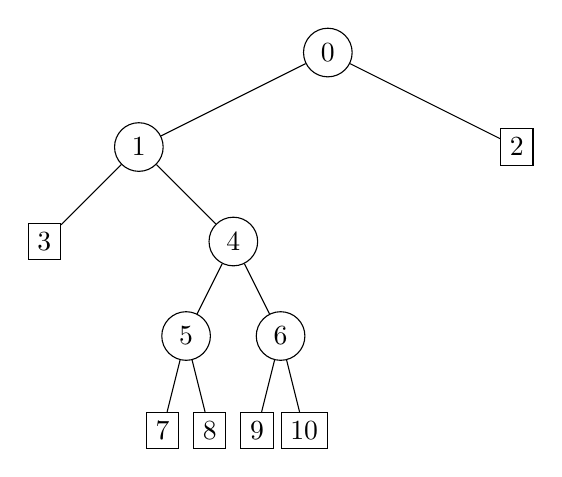
\begin{tikzpicture}[scale=0.3]
		\node[draw, circle] (0) at (0,0) {0};
		
		\node[draw, circle] (1) at (-8,-4) {1};
		\node[draw] (2) at (8,-4) {2};
		
		\node[draw] (3) at (-12,-8) {3};
		\node[draw, circle] (4) at (-4,-8) {4};
		
		\node[draw, circle] (5) at (-6,-12) {5};
		\node[draw, circle] (6) at (-2,-12) {6};
		
		\node[draw] (7) at (-7,-16) {7};
		\node[draw] (8) at (-5,-16) {8};
		\node[draw] (9) at (-3,-16) {9};
		\node[draw] (10) at (-1,-16) {10};
		
		\draw[-] (0) to node {} (1);
		\draw[-] (0) to node {} (2);
		\draw[-] (1) to node {} (3);
		\draw[-] (1) to node {} (4);
		\draw[-] (4) to node {} (5);
		\draw[-] (4) to node {} (6);
		\draw[-] (5) to node {} (7);
		\draw[-] (5) to node {} (8);
		\draw[-] (6) to node {} (9);
		\draw[-] (6) to node {} (10);
	\end{tikzpicture}
\end{center}

Quindi $n=5$ nodi interni e $6$ nodi esterni.\\

Usiamo un \textbf{array di $2n + 1$ bit} ($11$ in questo caso) e se il \textbf{nodo} è \textbf{interno} inserisco \textbf{1}, \textbf{altrimenti 0}. Per l'esempio precedente:
\begin{flalign*}
	\begin{array}{c c c c c c c c c c c}
		0 & 1 & 2 & 3 & 4 & 5 & 6 & 7 & 8 & 9 & 10 \\
	\end{array} \\
	\begin{array}{| c | c | c | c | c | c | c | c | c | c | c |}
		\hline
		1 & 1 & 0 & 0 & 1 & 1 & 1 & 0 & 0 & 0 & 0 \\
		\hline
	\end{array}
\end{flalign*}

\paragraph{Trovare i figli:} Voglio sapere dove sono i \textbf{figli di ogni nodo}. Per sapere tale indice per un nodo $p$ mi basta sapere quanti sono i nodi a destra del nodo considerato e quanti sono i nodi a sinistra del figlio di sinistra del nodo considerato, li sommo a $p$ e trovo l'indice del figlio.\\

I nodi totali dell'albero sono $2n+1$, i nodi interni $n$. I nodi interni prima di $p$ sono $ rank_b (p)$, quindi l'indice del figlio sinistro è 
$$ f_{sx} (p) = 2 rank_b (p) + 1 $$
$$ f_{dx} (p) = 2 rank_b (p) + 2 $$

\newpage

\paragraph{Trovare il genitore:} Ma chi è $p'$ tale che $p'$ è \textbf{genitore di} $p$? Non so se $p$ è il figlio di sinistra o destra, quindi varrà una di queste due proprietà
$$
\begin{array}{c c}
	2 rank (p') + 1 & = p \\
	2 rank (p') + 2 & = p
\end{array}
\implies rank (p') = \left\lfloor \frac{p}{2} - \frac{1}{2} \right\rfloor $$

Ma select è circa l'inverso di rank, quindi: 
$$
p' = select \left\lfloor \frac{p}{2} - \frac{1}{2} \right\rfloor
$$

Di conseguenza definiamo:
$$ parent(p) := select_b \left(\left\lfloor \frac{p}{2} - \frac{1}{2} \right\rfloor\right) $$

In questo modo tramite rank e select possiamo trovare sia padri che figli di un certo nodo all'interno dell'albero.\\

\paragraph{Dati satellite:} Ma se devo memorizzare \textbf{dati ausiliari} per ogni nodo oltre che la struttura?
\begin{itemize}
	\item Se i dati sono su \textbf{tutti i nodi} allora mi serve un vettore ausiliario di $2n+1$ \textbf{celle}.\\
	
	\item Se i dati sono \textbf{solo su i nodi interni} posso usare un vettore ausiliario con dimensione pari ai nodi interni e faccio una \textbf{rank per sapere la cella a cui accedere}.\\
\end{itemize}

\paragraph{Occupazione di memoria:} Dimensione dell'array: 
$$D_n = 2n + 1 + o(n)$$

L'\textbf{information theoretical lower bound} è 
$$ Z_n = 2n - o (\log n)$$

Quindi la struttura è \textbf{succinta} (considerando le precedenti strutture succinte per rank e select).\\

\newpage

\subsection{Codifica di Elias-Fano per sequenze monotone}
Elias-Fano è un modo \textbf{succinto} (compatto nel caso più generale, ma succinto in realtà) per \textbf{rappresentare delle sequenze crescenti}.\\

Partendo da una \textbf{sequenza di valori non decrescenti}
$$ x_1 \leq x_2 \leq x_3 \leq \, \dots \, \leq x_{n-1} < u $$

Si calcola un numero $\ell$ tale che
$$ \ell = \max \left\{0, \left\lfloor \log \frac{u}{n} \right\rfloor\right\} $$

Dividiamo in due parti la rappresentazione:
\begin{enumerate}
	\item Gli $\ell$ \textbf{bit inferiori} (meno significativi)
	$$ 
	\begin{array}{c c c}
		\ell_0 & = & x_0 \mod 2^\ell \\
		\ell_1 & = & x_1 \mod 2^\ell \\
		\vdots && \\
		\ell_{n-1} & = & x_{n-1} \mod 2^\ell \\
	\end{array}
	$$
	Vengono \textbf{memorizzati esplicitamente}.\\
	
	\item I \textbf{bit superiori} (più significativi)
	$$ \left\lfloor \frac{x_0}{2^\ell} \right\rfloor, \left\lfloor \frac{x_1}{2^\ell} \right\rfloor, \, \dots \, , \left\lfloor \frac{x_{n-1}}{2^\ell} \right\rfloor $$
	
	Vengono memorizzati come \textbf{differenza tra l'uno ed il successivo} ($\Delta$-compressione)
	$$ u_0, u_1, u_2, \, \dots $$
	Dove: 
	$$ u_i = \left\lfloor \frac{x_i}{2^\ell} \right\rfloor - \left\lfloor \frac{x_{i-1}}{2^\ell} \right\rfloor$$
	
	Con il presupposto che $x_{-1} =0$.\\
	Questi valori vengono \textbf{memorizzati in unario} in un unico vettore dove scrivo \textbf{tanti 0 quanti il valore}, \textbf{terminati da un 1}, esempio:
	$$ 3\; 7 \rightarrow 001 \; 0000001 $$
\end{enumerate}

\paragraph{Occupazione di spazio:} 
\begin{itemize}
	\item La \textbf{prima parte} richiede $\ell \cdot n$ \textbf{bit}, in quanto memorizzati esplicitamente.\\
	
	\item Per la \textbf{seconda parte} servono
	\begin{flalign*}
		\sum_{i=0}^{n-1} u_i + 1 & =  \sum_{i=0}^{n-1} \left(\left\lfloor \frac{x_1}{2^\ell}\right\rfloor - \left\lfloor \frac{x_{i-1}}{2^\ell}\right\rfloor + 1 \right) \\
		& = n + \sum_{i=0}^{n-1} \left(\left\lfloor \frac{x_1}{2^\ell}\right\rfloor - \left\lfloor \frac{x_{i-1}}{2^\ell}\right\rfloor\right) =
	\end{flalign*}
	
	E questa è una somma telescopica, quindi rimane solo 
	\begin{flalign*}
		= n + \frac{x_{n-1}}{2^\ell} - \frac{x_{-1}}{2^\ell} & = n + \frac{x_{n-1}}{2^\ell} \\
		& \leq n + \frac{u}{2^\ell} \\
		& = n + \frac{u}{2^{\left\lfloor \log \frac{u}{n} \right\rfloor}} \\
		& \leq n + \frac{u}{2^{\log \frac{u}{n} - 1}} \\
		& = n + \frac{2u}{u/n} \\
		& = 3n
	\end{flalign*}
	Quindi per la seconda parte \textbf{servono $3n$ bit}.\\
\end{itemize}

In \textbf{totale} servono:
\begin{flalign*}
	D_n & = \ell \cdot n + 3n \\
	& = (\ell + 3) n \\
	& = \left( \left\lfloor \log \frac{u}{n} \right\rfloor + 3 \right) n \\
	& = 2n + n \left\lceil \log \frac{u}{n}\right\rceil + o(n)
\end{flalign*}

Quindi un $ 2n + n \left\lceil \log \frac{u}{n}\right\rceil + o(n)$ bit.\\

\newpage

\paragraph{Trovare un valore:} Quindi per trovare il valore $x_i$ cosa faccio?\\
\begin{itemize}
	\item Per la \textbf{parte bassa} dei bit è facile in quanto è memorizzata esplicitamente. \\
	
	\item Per la \textbf{parte alta} faccio una select sul vettore che contiene tutte le parti alte in unario per trovare l'$i$-esimo 1:
	\begin{flalign*}
		select_{\underline u} (i) & = i + u_0 + u_1 + \, \dots \, + u_i \\
		& = i + \left\lfloor \frac{x_0}{2^\ell} \right\rfloor +  \left\lfloor \frac{x_1}{2^\ell} \right\rfloor -  \left\lfloor \frac{x_0}{2^\ell} \right\rfloor + \, \dots \, \\
		& = i + \left\lfloor \frac{x_i}{2^\ell} \right\rfloor
	\end{flalign*}
\end{itemize}

Trovate entrambe basta concatenare il valore.\\

\subsubsection{Information theoretical lower bound}

Fissati $n$ e $u$, \textbf{quante sono le possibili sequenze}
$$ 0 \leq x_0 \leq x_1 \leq \, \dots \, \leq x_{n-1} < u $$

Equivalente a dire: quanti possibili insiemi di cardinalità $n$ con ripetizioni ci sono? \\

Ancora equivalente al numero di soluzioni $\in \mathbb{N}^u$ di 
$$ c_0 + c_1 + \, \dots \, + c_{u-1} = n $$
Dove $c_i$ rappresenta quanti valori $i$ sono presenti nella sequenza iniziale.\\

Le soluzioni possiamo contarle con lo stars \& stripes counting:
\begin{itemize}
	\item Scriviamo $u-1$ barre
	\item Tra ogni barra e quella dopo poniamo $c_i$ stelle, quindi ci saranno $n$ stelle
\end{itemize}

\newpage

Quante sequenze di $n$ stelle e $u-1$ barre esistono?
\begin{flalign*}
	\left(\begin{array}{c}u+n-1 \\ u - 1\end{array}\right)
	& = \frac{(u+n-1)!}{(u-1)!(u+n-1-u+1)!} \\
	& = \frac{(u+n-1)!}{n! (u-1)!}
\end{flalign*}

Di conseguenza l'\textbf{information theoretical lower bound} è 
$$ Z_n = \log \left(\begin{array}{c}u+n-1 \\ u - 1\end{array}\right) = 
\log \left(\begin{array}{c}u+n-1 \\ n\end{array}\right)
$$

Ma sapendo che:
$$
\log \left(\begin{array}{c}
	A \\ B
\end{array}\right) \sim B \log \frac{A}{B} + (A - B) \log \frac{A}{A-B}
$$

E applicandola ponendo $A = u+n-1$ e $B = n$, quindi: 
$$ 
Z_n \sim n \log \frac{u+n-1}{n} + (u-1) \log \frac{u+n-1}{u-1}
$$

Ma considerando $u \gg n$ (l'universo molto più grande dei valori che effettivamente usiamo), quindi il secondo termine (da $u-1$) è tutto $\approx 1$, quindi:

$$ \approx n \log \frac{u}{n} \left( 1 + \frac{n}{u} - \frac{1}{u}\right)
= n \log \frac{u}{n} + n \log \left(1 + \frac{n}{u} - \frac{1}{u}\right)
$$

Sapendo che $x \approx \log (1 + x)$:
$$ Z_n \approx n \log \frac{u}{n}  + n \left(\frac{n}{u} - \frac{1}{u}\right)
\leq n \log \frac{u}{n} + \frac{n^2}{u}
$$
sempre considerando $n \ll u$.\\

\newpage

Riprendendo il $D_n$ di prima: 
$$ D_n = 2n + n \left\lceil \log \frac{u}{n}\right\rceil + o(n) $$

Che è dominato dal $2n$, quindi 
$$ D_n = O(Z_n) $$

La struttura quindi, in questo caso, non è succinta ma \textbf{compatta}.\\

Risulta compatta con assunzioni generiche, \textbf{supponendo che} $n \leq \sqrt{u}$, abbastanza sensata considerando che abbiamo presupposto che $u \gg n$, la struttura anziché compatta \textbf{diventa succinta}.\\

% End L21

\newpage

\subsection{Funzioni di Hash}

Su un universo $U$, una \textbf{funzione di hash} è 
$$ h: U \rightarrow m $$
dove $|U| > |m|$. Questa viene chiamata "funzione di hash per $U$ con $m$ \textbf{bucket}".\\

Requisiti di una funzione di hash $h$: 
\begin{enumerate}
	\item $h$ si deve calcolare in \textbf{tempo costante} (facile da calcolare).\\
	
	\item $h$ deve essere "molto iniettiva", non devono \textbf{esserci collisioni}, ma ci saranno per forza, quindi $h$ deve spargere bene gli elementi su $m$ bucket. Collision resistance, difficile trovare $h(x) = h(y)$ per $x \neq y$.\\
\end{enumerate}

Solitamente per le strutture dati si usa la "\textbf{full randomness assumption}", ovvero che la funzione di hash sia scelta in modo completamente casuale tra tutti i possibili, cosa che non regge nel mondo reale.\\

Quindi, di solito, si \textbf{restringe la quantità di funzioni di hash possibili}, in quanto, probabilmente, non serviranno tutte.\\

Considerando una funzione di hash 
$$ h: U \rightarrow 100$$

E stringhe richieste alla funzione della forma: 
$$ x = x_1 \, \dots \, x_n \in U $$

Quindi \textbf{scegliamo dei pesi}, con valore uniformemente a caso (qua possiamo farlo, questo è lo step fully random):
$$ w_1, \, \dots \, , w_{100}$$

\newpage

E \textbf{definiamo} la nostra \textbf{funzione di hash} come:
$$ h(x) := \left(\sum_{i=1}^{n} x_i \cdot w_i \right) \mod 100 $$
Ovvero il prodotto di ogni componente della stringa per il corrispondente peso.\\

In questo modo stiamo definendo una particolare \textbf{famiglia di funzioni di hash}, all'interno della quale posso scegliere uniformemente a caso
$$ \mathcal{H}_{U,m} \subseteq m^U $$

All'interno della quale vale la \textbf{proprietà}:
$$ \forall x \in U \;\;\;\; P [h(x) = t] = \frac{1}{m} \;\;\; \forall t \in m$$
Ovvero, all'interno della funzione i valori sono suddivisi equamente tra tutti i bucket possibili.\\

Quindi, non possiamo scegliere uniformemente a caso, quindi restringo l'universo a qualcosa che posso scegliere davvero uniformemente a caso.\\

\paragraph{Funzione di Hash Perfetta:} Una funzione di \textbf{hash è perfetta} per l'insieme $X$ iff è \textbf{iniettiva} su $X$ (è necessario che $m \geq |X|$, altrimenti è, ovviamente, impossibile).\\

\paragraph{Funzione di Hash minimale:} Si dice "\textbf{minimale}" la funzione di hash perfetta con il \textbf{numero di bucket minori possibili} per un dato universo, quindi con $|X| = m$.\\

\newpage

\subsubsection{Tecnica MWHC}

Per costruire una funzione di hash minimale. Dai nomi degli inventori: Majewski, Worwald, Hava\'s \& Czech.\\ %Wtf

L'obiettivo della tecnica è quello di ottenere una \textbf{funzione di hash minimale perfetta ordinata}, ovvero che permette di mappare i valori in un ordine preciso (order-preserving minimal perfect hash, opmpf per gli amici).\\
Questa tecnica può essere utilizzata per rappresentare funzioni statiche (generiche) ad $r$ bit, quindi un qualsiasi dizionario di valori statico.\\

Partendo da un \textbf{universo} $U$ ed un \textbf{insieme} $X \subseteq U$, \textbf{con} $|X| = n$; la \textbf{funzione} $f$ associa ad ogni \textbf{valore} $x_i \in X$ un \textbf{vettore} di $r$ bit
$$ f: X \rightarrow 2^r $$
I Bro ci hanno spiegato come memorizzare una funzione di questo tipo.\\

Primi \textbf{step}:
\begin{enumerate}
	\item \textbf{Fissano un} $m \geq n$
	\item Scelgono \textbf{uniformemente a caso due funzioni di hash }
	$$ h_1, h_2: U \rightarrow m $$
	\item Costruiscono un \textbf{grafo} dove
	\begin{itemize}
		\item i \textbf{vertici} sono i valori da $0$ a $m$, quindi $m$ vertici
		\item c'è un \textbf{arco} tra due nodi $i,j$ ogni volta che è presente una stringa tale che 
		$$x \in X, \;\;\;\; \{h_1(x), h_2(x)\} = \{i,j\} $$
		quindi tendenzialmente ci sono $n$ lati
	\end{itemize}
\end{enumerate}

\textbf{Situazioni spiacevoli:} 
\begin{itemize}
	\item $h_1(x) = h_2 (x)$ per qualche $x$, non vogliamo loop-de-loops
	\item $x,y \in X$, $x \neq y$ tali che $\{h_1 (x), h_2 (x)\} = \{h_1 (y), h_2 (y)\}$, in quanto vogliamo una corrispondenza 1 a 1 tra archi ed elementi di $X$
	\item il grafo è ciclico (vogliamo non lo sia), quindi per cercare di evitarlo scegliamo un $m$ "abbastanza grande"
\end{itemize}
Se ci si ritrova in una di queste situazioni si \textbf{cambia funzioni}. Questi eventi, con $m$ \textbf{abbastanza grande}, sono \textbf{poco probabili}.

\newpage

\addcontentsline{toc}{subsubsection}{\protect\numberline{}Teorema}
\paragraph{Teorema:} Con $m > 2.09n$, le funzioni $h_1, h_2$ hanno \textbf{quasi sempre} (asintoticamente) le \textbf{proprietà desiderate}, e il numero di \textbf{tentativi attesi} è circa $2$.\\

Ogni arco del grafo corrisponde ad un valore $x \in X$, di conseguenza ha associato un unico $f(x) \in 2^r$.\\

Possiamo creare un \textbf{sistema di equazioni} con $m$ variabili
$$ A[0], A[1], \, \dots \, , A[m-1] \in 2^r $$

Dove ci sono $x \in X$ \textbf{equazioni} della forma:
$$ \forall x \in X \;\;\;\; \left(A[h_1 (x)] + A[h_2(x)]\right) \mod 2^r = f(x) $$

Questo sistema \textbf{ammette soluzione} (grazie al fatto che il grafo è aciclico, ma non spiegheremo il perché, trust me bro) e memorizzo tali valori.\\

La \textbf{struttura dati contiene} le $m$ \textbf{variabili} e i \textbf{valori} $h_1,h_2$ e $m$.\\

\paragraph{Ma quando devo usare la struttura?} Calcolo
$$ f(v) = A[h_1(v)] + A[h_2 (v)] \mod 2^r $$
Ed è tempo costante, rispetto alla dimensione dell'input.\\

\paragraph{Quanto spazio occupa?}
\begin{itemize}
	\item la parte delle \textbf{funzioni di hash e $m$} occupa uno spazio che non dipende dai valori che vogliamo memorizzare quindi spazio \textbf{costante} $O(1)$ (che può essere o meno rilevante)
	\item le \textbf{variabili da memorizzare} occupano spazio in relazione alla dimensione di $r$, sono $m$ soluzioni, quindi in \textbf{totale} $m \cdot r$ bit.\\
\end{itemize}

Da notare che non stiamo memorizzando le chiavi, stiamo rappresentando una funzione a partire da dei valori definiti, se provo ad usare la struttura con una "chiave" non parte dell'insieme definito inizialmente funzionerà lo stesso, anche se non è detto che il risultato abbia senso.\\
%Maybe

\newpage

\subsubsection{Aciclicità $\rightarrow$ Peelability}
Questa costruzione si può avere anche su \textbf{ipergrafi}, usando \textbf{più funzioni di hash}, minimizzando il bound del valore $m$ a $1.23n$ con un 3-ipergrafo (3 funzioni di hash, ogni arco può collegare fino a 3 nodi); a salire di dimensioni aumenta il valore.\\

Con un \textbf{3-ipergrafo il teorema vale per} $m> \gamma n$, $\gamma = 1.23$.\\

Per un ipergrafo la nozione di aciclicità diventa "\textbf{peelability}".\\

Un ipergrafo $(V,E)$ \textbf{ammette una peeling sequence} iff esiste un modo per \textbf{ordinare gli iperarchi} $e_1, \, \dots \, , e_n \in E$ e una \textbf{sequenza di vertici} $x_1, \, \dots \, , x_n \in V$ in modo da avere una \textbf{sequenza}
$$
\begin{array}{c c}
	x_1, & e_1 \\
	x_2, & e_2 \\
	\vdots \\
	x_n, & e_n \\
\end{array}
$$
\textbf{tale che}: 
\begin{enumerate}
	\item $x_i \in e_i$, il lato si attacca a quel vertice (\textit{hinge})
	\item $x_i \notin e_j$ $\forall j < i$, ovvero andando avanti sono \textbf{sempre vertici nuovi}, non viene riusato lo stesso vertice
\end{enumerate}
In un grafo normale è facile vedere come una peeling sequence esista solo nel caso aciclico. Per il caso in più dimensioni te lo lascio immaginare, ma per un 3-ipergrafo è come "sbucciare" uno dei "piani" che uniscono i vertici (ovvero i lati) per volta, senza toccare nodi vecchi.\\

\newpage

\paragraph{Spazio occupato:} Per la costruzione con MWHC su un 3-ipergrafo 
$$ \gamma n r \; \text{ bit}$$

Ma molte entry nel vettore delle soluzioni potrebbero non essere necessarie (se non presenti nel sistema di equazioni possono essere poste a 0), quindi posso \textbf{memorizzare solo i valori utili} (entry non zero), più un vettore di bit per memorizzare la posizione, su cui bisogna fare rank e select per trovare gli indici giusti.\\

Quindi la \textbf{versione compressa} occupa:
$$ n r + \gamma n + o(n) $$

Che \textbf{conviene quando} 
$$ n r + \gamma n < \gamma n r \implies r > 5$$
per $\gamma = 1.23$.\\

% End L22
%Fine del corso :(